\documentclass{letter}
\usepackage{enumitem}
\usepackage{mathtools}
\usepackage{fancyhdr}
\usepackage{xcolor}
\usepackage{mdframed}
\usepackage{bm}
\usepackage[letterpaper,portrait,left=2cm,right=2cm,top=3.5cm,bottom=2cm]{geometry}
\pagestyle{fancy}

\fancyhf{}
\rhead{Robert Wagner\\June 11, 2016}
\lhead{Math 2101\\Assignment 3}
\newcounter{question}
\setcounter{question}{0}
\usepackage{amsmath,amsthm}
\usepackage{amssymb}
\usepackage{tikz}
\usetikzlibrary{arrows}


% magnitude bars
\newcommand{\norm}[1]{\lvert #1 \rvert}

% explicit vector
\newcommand{\Ve}[1]{\langle #1 \rangle}

% named vector
\newcommand{\Vn}[1]{\vec{\bm{#1}}}

% a line with an arrow above
\newcommand{\Line}[1]{\overrightarrow{#1}}

% equals with question mark above
\newcommand{\?}{\stackrel{?}{=}}

% formatting for questions
\newcommand\Que[1]{%
   \leavevmode\noindent
   #1
}

% formatting for answers
\newcommand\Ans[2][]{%
   \leavevmode\noindent
   {
       \begin{mdframed}[backgroundcolor=blue!10]
       #2
       \end{mdframed}
   }
}

% this is like align but squashed     
\newenvironment{salign}
 {\par$\!\aligned}
 {\endaligned$\par}

% a matrix, parameter is column count
\newenvironment{Mat}[1]{%
  \left[\begin{array}{*{#1}{r}}
}{%
  \end{array}\right]
}

% an augmented matrix, parameter is non-augmented column count
\newenvironment{Amat}[1]{%
  \left[\begin{array}{@{}*{#1}{r}|r@{}}
}{%
  \end{array}\right]
}

\begin{document}


\begin{enumerate}
    \item Given any point $P=(x,y)$, we can define a  \textbf{transformation} $(x,y) \to (x',y')$, where
    \begin{align*}
      ax+by &= x' \\
      cx+dy &= y'
    \end{align*}
    for some real numbers $a,b,c,d$.  We write $T:P\to P'$\ to indicate $P'$ is the point $(x',y')$\ produced by applying the transformation $T$\ to the point $P$; We also write $TP=P$.  In the following, you don't have to draw a picture ... but it will probably help.
    \begin{enumerate}[label=(\alph*)]
        \item\Que{
          Write down the linear transformation corresponding to the geometric transformation of reflecting a point across the $x$-axis.  (In other words, find $a,b,c,d$\ so that $(x',y')$\ is the reflection of $(x,y)$\ across the $x$-axis)  Then write the corresponding coefficient matrix (call this matrix $M_x$).
           
        }
        \Ans{
          \begin{minipage}[m]{0.6\textwidth}
            \centering
            \begin{tikzpicture}[x=1cm,y=1cm]
                \draw[<->](-2,0)--(2,0);
                \draw[<->](0,-2)--(0,2);
                \node[label={0:{$P=(x,y)$}}] (P) at (1,1.5) {\textbullet};
                \node[label={0:{$P'=(x,-y)$}}] (P') at (1,-1.5) {\textbullet};          
                \draw[->] (1,1.5) (P) to [bend left] (P'); 
            \end{tikzpicture}
          \end{minipage}
          \begin{minipage}[m]{0.6\textwidth}
            \begin{salign}
             x'&=1x+0y\\
             y'&=0x-1y\\
             M_x&=
             \begin{Mat}{2}
               1 & 0 \\
               0 & -1
             \end{Mat}\\
             M_xP&=P'
            \end{salign}
          \end{minipage}
        }    
        \item \Que{Write down the linear transformation corresponding to the geometric transformation of rotating the point $(x,y)$\ $90^{\circ}$ counter-clockwise around the origin.  Then write the corresponding coefficient matrix (call this matrix $R_{90}$).
        }
        \Ans{
            \begin{minipage}[m]{0.6\textwidth}
            \centering
            \begin{tikzpicture}[x=1cm,y=1cm]
                \draw[<->](-2,0)--(2,0);
                \draw[<->](0,-2)--(0,2);
                \node[label={0:{$Q=(x,y)$}}] (Q) at (1.5,0.5) {\textbullet};
                \node[label={180:{$Q'=(-y,x)$}}] (Q') at (-0.5,1.5) {\textbullet};          
                \draw[->] (Q) to [bend right] (Q'); 
            \end{tikzpicture}
          \end{minipage}
          \begin{minipage}[m]{0.6\textwidth}
            \begin{salign}
             x'&=0x-1y\\
             y'&=1x+0y\\
             R_{90}&=
             \begin{Mat}{2}
               0 & -1 \\
               1 & 0
             \end{Mat}\\
             R_{90}Q&=Q'
            \end{salign}
          \end{minipage}
        }
        \item \Que{Write down the linear transformation corresponding to the geometric transformation of reflecting the point $(x,y)$\ across the $x$-axis, followed by rotating the point $90^{\circ}$\ counter-clockwise around the origin.  Then write the corresponding coefficient matrix (call this matrix $T$).
        }
        \Ans{
             \begin{minipage}[m]{0.6\textwidth}
            \centering
            \begin{tikzpicture}[x=1cm,y=1cm]
                \draw[<->](-2,0)--(2,0);
                \draw[<->](0,-2)--(0,2);
                \node[label={0:{$R=(x,y)$}}] (R) at (0.5,1.5) {\textbullet};
                \node[label={0:{$(x,-y)$}}] (R') at (0.5,-1.5) {\textbullet};
                \node[label={0:{$R'=(y,x)$}}] (R'') at (1.5,0.5) {\textbullet};          
                \draw[->] (R) to [bend left] (R');
                \draw[->] (R') to [bend right] (R''); 
            \end{tikzpicture}
          \end{minipage}
          \begin{minipage}[m]{0.6\textwidth}
            \begin{salign}
             x'&=0x+1y\\
             y'&=1x+0y\\
             T&=
             \begin{Mat}{2}
               0 & 1 \\
               1 & 0
             \end{Mat}\\
             R_{90}M_xR &=TR=R'
            \end{salign}
          \end{minipage}
        }
        \newpage
        \item \Que{
            Suppose $S, T$\ are two linear transformations, and $P$\ is a point.  Define $M=S+T$\ and remember \textbf{we haven't yet defined matrix addition} (so even if you know how to add two matrices, you may not use this knowledge).  Show that if we want the distributive law $(S+T)P = SP+TP$\ to hold, we must define $m_{ij}=s_{ij}+t_{ij}$.
        }
        \Ans{
        Let $P=(x,y)$, 
            $S = \begin{Mat}{2} a & b \\ c & d \end{Mat}$,
            and  
            $T=\begin{Mat}{2} e & f \\ g & h \end{Mat}$.
            Then 
            \begin{align*}
              SP+TP &= \begin{Mat}{2} a & b \\ c & d \end{Mat}\Ve{x , y} +
                       \begin{Mat}{2} e & f \\ g & h \end{Mat}\Ve{x , y} \\
                    &= \Ve{ax+by , cx+dy} +  \Ve{ex+fy , gx+hy} \\
                    &= \Ve{(a+e)x + (b+f)y, (c+g)x+(d+h)y} \\
                    &= \begin{Mat}{2} a+e & b+f \\ c+g & d+h \end{Mat}\Ve{x,y}
                     = (S+T)P            
            \end{align*}
            Therefore it follows in the two dimensional case that for $M=S+T$, matrix addition defined as $m_{ij}=s_{ij}+t_{ij}$\ will hold the distributive property. 
        }
    \end{enumerate}
    ~\\
    \item 
        If $A,B$\ are the matrices corresponding to a geometric transformation, we interpret the matrix product $AB$\ as the geometric transformation produced by applying $B$ first, then applying $A$.  
    \begin{enumerate}[label=(\alph*)]
    \item \Que{
        Is matrix multiplication commutative? (In other words, given two matrices $A, B$, will $AB = BA$?)  Explain your conclusion.
    }
    \Ans{
    No, since we can see from the geometric transformation example that $R_{90}M_x \not= M_xR_{90}$, and in general it is not necessarily true for any matrices $A,B$\ since $A$\ is treated as a set of row vectors, and $B$\ is treated as a set of column vectors such that for $M=AB$, 
    \[
        m_{ij} = \Vn{a}_i \cdot \Vn{b}_j
    \]
    for all rows $i \in A$\ and columns $j \in B$. \\
    In general, if $A=A^T$\ and $B=B^T$\ then $AB=BA$.
    }
    \item \Que{
        Find $R_{90}M_x$.  
    }
    \Ans{
         From item 1(c) above, we see that
         \[
         R_{90}M_x = T =
         \begin{Mat}{2}
           0 & 1 \\
           1 & 0
         \end{Mat}
         \]
    }
    \item \Que{
        It's tempting to define the product of two matrices componentwise:
        \begin{align*}
            \begin{Mat}{2}
              a & b \\
              c & d
            \end{Mat}
            \begin{Mat}{2}
              m & n \\
              p & q
            \end{Mat}     
            \?
            \begin{Mat}{2}
              am & bn \\
              cp & dq
            \end{Mat}       
        \end{align*}
        Show that this definition does not calculate $R_{90}M_x$\ correctly.  
    }
    \Ans{
      \begin{align*}
        R_{90}M_x = 
        \begin{Mat}{2}
          0 & -1 \\
          1 & 0
        \end{Mat}
        \begin{Mat}{2}
          1 & 0 \\
          0 & -1
        \end{Mat}        
        =
        \begin{Mat}{2}
          0 \cdot 0 & -1\cdot 0 \\
          1 \cdot 0 & -1\cdot 0  
        \end{Mat}
        =
        \begin{Mat}{2}
          0 & 0 \\
          0 & 0
        \end{Mat}
        \not= T
      \end{align*}
    }
    \newpage
    \item \Que{
        We actually find the product of $2\times 2$ matrices as
        \begin{align*}
             \begin{Mat}{2}
              a & b \\
              c & d
            \end{Mat}
            \begin{Mat}{2}
              m & n \\
              p & q
            \end{Mat}     
            =
            \begin{Mat}{2}
              am+bp & ab+bq \\
              cm+dp & cn+dq
            \end{Mat}   
        \end{align*}
        Show that this definition gives us $T=R_{90}M_x$.
    }
    \Ans{
      \begin{align*}
        R_{90}M_x = 
        \begin{Mat}{2}
          0 & -1 \\
          1 & 0
        \end{Mat}
        \begin{Mat}{2}
          1 & 0 \\
          0 & -1
        \end{Mat}        
        =
        \begin{Mat}{2}
          (0 \cdot 1) + (-1\cdot 0) & (0\cdot 0) + (-1\cdot -1) \\
          (1 \cdot 1) + (0\cdot 0)  & (1\cdot 0) + (0\cdot -1)  
        \end{Mat}
        =
        \begin{Mat}{2}
          0 & 1 \\
          1 & 0
        \end{Mat}
        = T
      \end{align*}
    }
    
    \item \Que{
       Use matrix multiplication as defined above to find $T'=M_xR_{90}$.  Then verify that this is correct, by identifying the geometric transformation to the product $M_xR_{90}$\ and finding the corresponding linear transformation.
    }    
    \Ans{
    \begin{align*}
        M_xR_{90} = 
        \begin{Mat}{2}
          1 & 0 \\
          0 & -1
        \end{Mat}
        \begin{Mat}{2}
          0 & -1 \\
          1 & 0
        \end{Mat}        
        =
        \begin{Mat}{2}
          (1 \cdot 0) + (0\cdot 1) & (1\cdot -1) + (0\cdot 0) \\
          (0 \cdot 0) + (-1\cdot 1)  & (0\cdot -1) + (-1\cdot 0)  
        \end{Mat}
        =
        \begin{Mat}{2}
          0 & -1 \\
          -1 & 0
        \end{Mat}
        = T'
      \end{align*}
    \begin{minipage}[m]{0.6\textwidth}
            \centering
            \begin{tikzpicture}[x=1cm,y=1cm]
                \draw[<->](-2,0)--(2,0);
                \draw[<->](0,-2)--(0,2);
                \node[label={0:{$S=(x,y)$}}] (S) at (0.5,1.5) {\textbullet};
                \node[label={180:{$(-y,x)$}}] (S') at (-1.5,0.5) {\textbullet};
                \node[label={180:{$S'=(-y,-x)$}}] (S'') at (-1.5,-0.5) {\textbullet};          
                \draw[->] (S) to [bend right] (S');
                \draw[->] (S') to [bend left] (S''); 
            \end{tikzpicture}
          \end{minipage}
          \begin{minipage}[m]{0.6\textwidth}
            \begin{salign}
            \text{verify:}\\
             x'&=0x-1y\\
             y'&=-1x+0y\\
             T'&=
             \begin{Mat}{2}
               0 & -1 \\
               -1 & 0
             \end{Mat}\\
             M_xR_{90}S &=T'S=S'
            \end{salign}
          \end{minipage}
    }
    \end{enumerate}
    ~\\
    \item Let 
        $M= \begin{Mat}{3}
            1/2 & 1/4 & 1/2 \\
            0   & 1/4 & 1/2 \\
            m_{31} & 1/2 & m_{33}
            \end{Mat}$
         be a stochasic matrix.  
    \begin{enumerate}[label=(\alph*)]        
    \item \Que{
        Interpret this as a set of movement rules between three locations by identifying what fractions of those at each location at $t=k$\ will move to the other locations at $t=k+1$.
    }
    \Ans{
      \begin{itemize}
        \item $1/2$ of those at location $a$ move to location $c$.
        \item $1/4$ of those at location $b$ move to location $a$, and $1/2$ move to location $c$.
        \item $1/2$ of those at location $c$ move to location $a$, and $1/2$ move to location $b$. 
      \end{itemize}
    }
    \item \Que{
        Find $m_{31}$\ and $m_{33}$.
    }
    \Ans{
      Since each columns must sum to one, it follows that \\
      \begin{minipage}[m]{0.4\textwidth}
      
      \begin{align*}
      m_{11}+m_{21}+m_{31}&=1 \\
      1/2+0+m_{31}        &=1\\
      m_{31}              &=\underline{1/2}
      \end{align*}
      \end{minipage}
      \begin{minipage}[m]{0.4\textwidth}
      
      \begin{align*}
      m_{31}+m_{32}+m_{33}&=1 \\
      1/2 + 1/2 + m_{33}&=1   \\
      m_{33} &= \underline{0}
      \end{align*}
      \end{minipage}
    }
    \newpage
    \item \Que{
        Find $M^2$, where $m_{ij}$\ corresponds to the fraction of those in location $i$\ at $t=k$\ who will be in location $j$\ at $t=k+2$.  
    }
    \Ans{
     \begin{center}
          \begin{tabular}{| l || c | c | c |} 
            \hline
            & $a$ & $b$ & $c$ \\ [0.5ex] 
            \hline\hline
            $t=k$ & $a_k$ & $b_k$ & $c_k$ \\ [0.5ex]
            \hline
            $t=k+1$ & $\frac{a_k}{2}+\frac{b_k}{4}+\frac{c_k}{2}$ & 
                      $\frac{b_k}{4}+\frac{c_k}{2}$ & $\frac{a_k}{2}+\frac{b_k}{2}$ \\ [0.5ex]
            \hline
            $t=k+2$ & $\frac{\frac{a_k}{2}+\frac{b_k}{4}+\frac{c_k}{2}}{2} + 
                       \frac{\frac{b_k}{4}+\frac{c_k}{2}}{4} +
                       \frac{\frac{a_k}{2}+\frac{b_k}{2}}{2}$ & 
                      $\frac{\frac{b_k}{4}+\frac{c_k}{2}}{4} + 
                       \frac{\frac{a_k}{2}+\frac{b_k}{2}}{2}$ & 
                      $\frac{\frac{a_k}{2}+\frac{b_k}{4}+\frac{c_k}{2}}{2} + 
                       \frac{\frac{b_k}{4}+\frac{c_k}{2}}{2}$ \\ [0.5ex]
            \hline
          \end{tabular}
        \end{center}
        \begin{align*}
        a_{k+2}  &= \frac{a_{k+1}}{2}+\frac{b_{k+1}}{4}+\frac{c_{k+1}}{2} 
                  = \frac{\frac{a_k}{2}+\frac{b_k}{4}+\frac{c_k}{2}}{2} + 
                       \frac{\frac{b_k}{4}+\frac{c_k}{2}}{4} +
                       \frac{\frac{a_k}{2}+\frac{b_k}{2}}{2} \\
                 &= \frac{2a_k+b_k+2c_k}{8}+\frac{b_k+2c_k}{16}+\frac{a_k+b_k}{4} \\
                 &= \frac{4a_k+2b_k+4c_k+b_k+2c_k+4a_k+4b_k}{16} \\
                 &= \frac{8a_k+7b_k+6c_k}{16} 
                 = \frac{a_k}{2} + \frac{7b_k}{16} + \frac{3c_k}{8} \\
        b_{k+2}  &= \frac{b_{k+1}}{4} + \frac{c_{k+1}}{2} 
                 = \frac{\frac{b_k}{4}+\frac{c_k}{2}}{4} + 
                       \frac{\frac{a_k}{2}+\frac{b_k}{2}}{2} 
                 = \frac{b_k+2c_k}{16}+\frac{a_k+b_k}{4} \\
                 &= \frac{4a_k+5b_k+2c_k}{16} 
                 = \frac{a_k}{4}+\frac{5b_k}{16}+\frac{c_k}{8}  \\
        c_{k+2}  &= \frac{a_{k+1}}{2}+\frac{b_{k+1}}{4}+\frac{c_{k+1}}{2}
                  = \frac{\frac{a_k}{2}+\frac{b_k}{4}+\frac{c_k}{2}}{2} + 
                       \frac{\frac{b_k}{4}+\frac{c_k}{2}}{2} \\
                 &=\frac{2a_k+b_k+2c_k}{8} + \frac{b_k+2c_k}{8}
                 =\frac{a_k}{4} + \frac{b_k}{4} + \frac{c_k}{2}    
        \shortintertext{therefore}
        M^2 &= \begin{Mat}{3}
                 1/2 & 7/16 & 3/8 \\
                 1/4 & 5/16 & 1/8 \\
                 1/4 & 1/4  & 1/2 
               \end{Mat}                 
        \end{align*}                          
    }
    \item \Que{
      Explain how you found the number of people in location $c$ at $t=k+2$.  
    } 
    \Ans{
        First, we find $c_{k+1}= Mc_k =$\ the number of people at location $c$\ at time $k+1$ by applying the matrix $M$\ to $c_k$. Then apply the matrix $M$ to $c_{k+1}$\ to find $c_{k+2}$. 
        }
    \item \Que{
      The preceeding problem suggests that if $A, B$\ are $2 \times 2$\ matrices, the product $AB$\ is the matrix whose entries correspond to the dot product of the rows of $A$\ with the columns of $B$.  Verify that this works on $3\times 3$\ matrices.
    }
    \Ans{
      Let $A = \begin{Mat}{3} 
                   a_{11} & a_{12} & a_{13} \\
                   a_{21} & a_{22} & a_{23} \\
                   a_{31} & a_{32} & a_{33}
               \end{Mat}$\ 
          and 
          $B = \begin{Mat}{3}
                   b_{11} & b_{12} & b_{13} \\
                   b_{21} & b_{22} & b_{23} \\
                   b_{31} & b_{32} & b_{33}
               \end{Mat}$. 
          \begin{align*}
          \text{Thus } AB &=
                  \begin{Mat}{3}
                    a_{11}b_{11}+a_{12}b_{21}+a_{13}b_{31} & 
                    a_{11}b_{12}+a_{12}b_{22}+a_{13}b_{32} &
                    a_{11}b_{13}+a_{12}b_{23}+a_{13}b_{33} \\
                    a_{21}b_{11}+a_{22}b_{21}+a_{23}b_{31} &
                    a_{21}b_{12}+a_{22}b_{22}+a_{23}b_{32} &
                    a_{21}b_{13}+a_{22}b_{23}+a_{23}b_{33} \\
                    a_{31}b_{11}+a_{32}b_{21}+a_{33}b_{31} &
                    a_{31}b_{12}+a_{32}b_{22}+a_{33}b_{32} &
                    a_{31}b_{13}+a_{32}b_{23}+a_{33}b_{33}
                  \end{Mat} \\
                  &=
                  \begin{Mat}{3}
                   \Vn{a_1} \cdot \Vn{b_1} & \Vn{a_1} \cdot \Vn{b_2} & \Vn{a_1} \cdot \Vn{b_3} \\
                   \Vn{a_2} \cdot \Vn{b_1} & \Vn{a_2} \cdot \Vn{b_2} & \Vn{a_2} \cdot \Vn{b_3} \\
                   \Vn{a_3} \cdot \Vn{b_1} & \Vn{a_3} \cdot \Vn{b_2} & \Vn{a_3} \cdot \Vn{b_3}
                 \end{Mat}
            \end{align*}     
          Thus $AB_{ij}=\Vn{a_i}\cdot\Vn{b_j}$\ where $\{\Vn{a_i}\}_{i\in I}$\ are the rows of $A$, and $\{\Vn{b_j}\}_{j\in J}$\ are the columns of $B$ where $I,J=\{1,2,3\}$.           
                 
    }
    \end{enumerate}
    \newpage
    \item 
      The identity transformation is simply $(x,y) \to (x,y)$.  We'll continue to use $M_x$\ and $R_{90}$\ from above.
    \begin{enumerate}[label=(\alph*)]
    \item \Que{
        Write down the coefficient matrix corresponding to the identity transformation.    
    }
    \Ans{
    \[
      I = \begin{Mat}{2} 1 & 0 \\ 0 & 1 \end{Mat}
    \]
    }
    \item \Que{
        Given a matrix $B$, the inverse matrix $B^{-1}$\ satisfies $B^{-1}B = I$.  First, describe the geometric transformation corresponding to the matrix $M_x^{-1}$, then find $M_x^{-1}$.
    }
    \Ans{
        Since $M_x\Ve{x,y}=\Ve{x,-y}$, We should define $M_x^{-1}$\ such that $M_x^{-1}\Ve{x,-y} = \Ve{x,y}$.  In the case of a mirroring transformation like $M_x$, we can see that $M_xM_x=I$ since 
        \begin{align*}
           M_xM_x\Ve{x,y}&=M_x\Ve{x,-y}\\&=\Ve{x,y}
         \shortintertext{therefore}
           M_x^{-1}&=M_x
         \end{align*} 
    }
    \item \Que{
        Explain, without computing or otherwise referring to the values of the matrices involved, why $R_{90}^3=R_{90}^{-1}$.    
    }
    \Ans{
        
        Since $R_{90}^4P = P$\ it follows that $R_{90}^4 = I$\ therefore
        \begin{align*}
        R_{90}^{-1}R_{90}^4&=R_{90}^{-1}I \\
        R_{90}^3&=R_{90}^{-1}    
        \end{align*}
        
        \begin{minipage}[m]{0.6\textwidth}
            \centering
            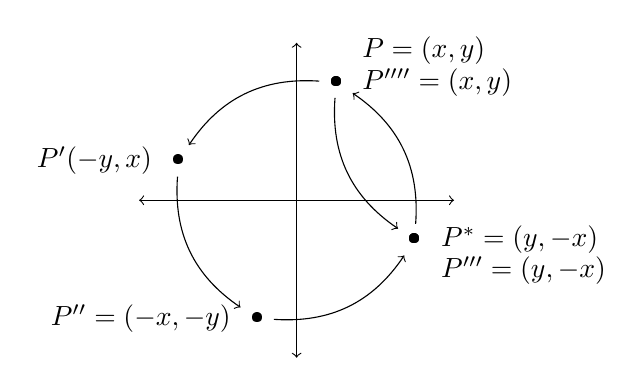
\begin{tikzpicture}[x=1cm,y=1cm]
                \draw[<->](-2,0)--(2,0);
                \draw[<->](0,-2)--(0,2);
                \node[label={25:{$P=(x,y)$}}] (P) at (0.5,1.5) {\textbullet};
                \node[label={180:{$P'(-y,x)$}}] (P') at (-1.5,0.5) {\textbullet};
                \node[label={180:{$P''=(-x,-y)$}}] (P'') at (-0.5,-1.5) {\textbullet};
                \node[label={-25:{$P'''=(y,-x)$}}] (P''') at (1.5,-0.5) {\textbullet};   
                \node[label={0:{$P^*=(y,-x)$}}] (P*) at (1.5,-0.5) {\textbullet};
                \node[label={0:{$P''''=(x,y)$}}] (P'''') at (0.5,1.5) {\textbullet};       
                \draw[->] (P) to [bend right] (P');
                \draw[->] (P') to [bend right] (P'');
                \draw[->] (P'') to [bend right] (P''');
                \draw[->] (P''') to [bend right] (P); 
                \draw[->] (P) to [bend right] (P*);
            \end{tikzpicture}
          \end{minipage}
          \begin{minipage}[m]{0.6\textwidth}
            \begin{salign}
             R_{90}^3P &= P''' \\
             x'''&=0x+1y \\
             y'''&=-1x+0y \\
             R_{90}^{-1}P &= P^* \\
             x^*&=0x+1y\\
             y^*&=-1x+0y\\
             R_{90}^{-1}P &=R_{90}^3P
            \end{salign}
          \end{minipage}
    }
    \item \Que{
        Find $R_{90}^{-1}$.      
    }
    \Ans{
      By the answer above, $R_{90}^{-1}=\begin{Mat}{2} 0 & 1 \\ -1 & 0 \end{Mat}$.
      }
    \item \Que{
    Suppose $A, B$\ are matrices corresponding to some geometric transformations.  \\What is $(AB)^{-1}$?  Explain.
    }
    \Ans{
    For some matrices $A, B$\ such that $T=AB$, the inverse $T^{-1} = (AB)^{-1}$\ is the matrix such that $T^{-1}T=(AB)^{-1}AB=I$.
    \begin{align*}
        &(AB)^{-1}AB&&=I \\
        &(AB)^{-1}ABB^{-1}      &&= IB^{-1}=B^{-1}\\
        &(AB)^{-1}AI&&=(AB)^{-1}A = B^{-1}\\
        &(AB)^{-1}AA^{-1}       &&= B^{-1}A^{-1} \\
        &(AB)^{-1}I &&= (AB)^{-1} = \underline{B^{-1}A^{-1}}
    \end{align*}
    }
    \end{enumerate}
    ~~\\
    \item Answer the following questions.
    \begin{enumerate}[label=(\alph*)]
    \item \Que{
    Reduce the following matrix to row echelon form:
    \[\begin{Amat}{3} 3 & 1 & 5 & 1 \\ 2 & -1 & 3 & -2 \\ 1 & 4 & 0 & 3 \end{Amat}\]
    }
    \Ans{
      \begin{salign}
        & ~~~~~ R_1-R_2 \to R_1  \\
        & ~~~~~ R_2-2R_3 \to R_2 \\
        & ~~~~~ R_3-R_1 \to R_3 ~~~~~~~~~~~ 9R_3+2R_2 \to R_3 ~~~~~~~~~~~\text{normalize}~~\\
        \begin{Amat}{3} 
            3 & 1 & 5 & 1 \\ 
            2 & -1 & 3 & -2 \\ 
            1 & 4 & 0 & 3 
        \end{Amat}
        &=
        \begin{Amat}{3} 
            1 & 2 & 2 & 3 \\ 
            0 & -9 & 3 & -8 \\ 
            0 & 2 & -2 & 0 
        \end{Amat}
        =
        \begin{Amat}{3}
            1 & 2 & 2 & 3 \\
            0 & -9 & 3 & -8 \\
            0 & 0 & -12 & -16
        \end{Amat}
        =
        \begin{Amat}{3}
            1 & 2 & 2 & 3 \\
            0 & 1 & -1/3 & 8/9 \\
            0 & 0 & 1 & 4/3
        \end{Amat}
      \end{salign}
    }
    \item \Que{
    Let $\Vn{u}=\Ve{u_1,u_2,u_3}$\ and $\Vn{v}=\Ve{v_1,v_2,v_3}$.  Prove or disprove: 
        $\norm{\Vn{u}+\Vn{v}} \leq \norm{\Vn{u}} + \norm{\Vn{v}}$.   
    }
    \Ans{
      Note that $a\leq b$\ if and only if $a^2\leq b^2$\ for all $a,b \in [0,\infty)$.  Also note that $\norm{\Vn{u}+\Vn{v}} \in [0,\infty)$, and that $\norm{\Vn{u}}, \norm{\Vn{v}} \in [0,\infty)$.\\
      Let $a=\norm{\Vn{u}+\Vn{v}}$, $b=\norm{\Vn{u}}+\norm{\Vn{v}}$, and $\theta \in [0,\pi]$ be the angle between $\Vn{u}, \Vn{v}$.  Thus
      \begin{align*}
        a^2 &= \left(\sqrt{(u_1+v_1)^2 + (u_2+v_2)^2 + (u_3+v_3)^2}\right)^2 \\
          &= (u_1^2+2u_1v_1+v_1^2) + (u_2^2+2u_2v_2+v_2^2) + (u_3^2+2u_3v_3+v_3^2) \\
          &= (u_1^2+u_2^2+u_3^2) + (v_1^2+v_2^2+v_3^2) + 2(u_1v_1+u_2v_2+u_3v_3) \\
          &= \norm{\Vn{u}}^2 + \norm{\Vn{v}}^2 + 2(\Vn{u}\cdot\Vn{v})
           = \norm{\Vn{u}}^2 + \norm{\Vn{v}}^2 + 2\left(\norm{\Vn{u}}\norm{\Vn{v}}\cos\theta\right) \\   
        b^2 &= \left(\sqrt{u_1^2+u_2^2+u_3^2}+\sqrt{v_1^2+v_2^2+v_3^2}\right)^2 \\
          &= \left(\sqrt{u_1^2+u_2^2+u_3^2}\right)^2 + 
             2\sqrt{(u_1^2+u_2^2+u_3^2)(v_1^2+v_2^2+v_3^2)} +
             \left(\sqrt{v_1^2+v_2^2+v_3^2}\right)^2 \\
          &= \norm{\Vn{u}}^2 + \norm{\Vn{v}}^2 + 2\norm{\Vn{u}}\norm{\Vn{v}}
      \intertext{
          Since $-1\leq\cos\theta\leq 1$\ 
          it follows that 
          $2\norm{\Vn{u}}\norm{\Vn{v}}\cos\theta \leq 2\norm{\Vn{u}}\norm{\Vn{v}}$, thus          
          }
         &\norm{\Vn{u}}^2 + \norm{\Vn{v}}^2 + 2\norm{\Vn{u}}\norm{\Vn{v}}\cos\theta \leq 
         \norm{\Vn{u}}^2 + \norm{\Vn{v}}^2 + 2\norm{\Vn{u}}\norm{\Vn{v}} \text{ thus } 
         a^2 \leq b^2
      \shortintertext{and subsequently}
         &a \leq b \text{ thus }
         \norm{\Vn{u}+\Vn{v}} \leq \norm{\Vn{u}}+\norm{\Vn{v}} \text{ for all vectors }\Vn{u},\Vn{v} \in \mathbb{R}^3.
      \qed\end{align*}
     
    }
    \item \Que{
    Let $\Vn{u}=\Ve{u_1,u_2,u_3}$\ and $\Vn{v}=\Ve{v_1,v_2,v_3}$.  Prove or disprove:
        $\Vn{u}\cdot\Vn{v} = \Vn{v}\cdot\Vn{u}$.
    }
    \Ans{
       \begin{align*}
           \Vn{u}\cdot\Vn{v} &= u_1v_1+u_2v_2+u_3v_3 \\
         \shortintertext{since $ab=ba$\ for all $a,b \in \mathbb{R}$\ it follows that}            
           u_1v_1+u_2v_2+u_3v_3  &= v_1u_1+v_2u_2+v_3u_3
         \shortintertext{and subsequently}  
           \Vn{u}\cdot\Vn{v} &= \Vn{v}\cdot\Vn{u}
           \qed
       \end{align*}
    }
    \newpage
    \item \Que{
    Let $\Vn{p}=\Ve{3,-1,1}$.  Find all vectors that are perpendicular to $\Vn{p}$.    
    }
    \Ans{
        Let $\Vn{u} = \Ve{u_1,u_2,u_3}$\ such that $\Vn{p}\cdot\Vn{u}=0$.  Thus
        \begin{align*}
            \Vn{p}\cdot\Vn{u}=3u_1+(-1)u_2+1u_3 &= 0
        \shortintertext{To parameterize, let}
            u_2 &= 3s\\
            u_3 &= 3t
        \shortintertext{It follows through substitution that}
           3u_1 + (-1)(3s)+(3t) &= 0 \\
           3u_1 &= 3s-3t \\
            u_1 &= s-t\\
        \shortintertext{Thus we can write}
            U=\{\Vn{u}\in\mathbb{R}^3:\Vn{u}=s\Ve{1,3,0}+t\Ve{-1,0,3} \text{ for all }s,t \in \mathbb{R}\}        
        \end{align*}
        Therefore the set $U$ is a plane containing all vectors perpendicular to $\Vn{p}$.
    }
    \end{enumerate}
\end{enumerate} 
\end{document}  